\documentclass[a4paper]{article}
\usepackage[english,russian]{babel}
\usepackage{multicol}
\usepackage[12pt]{extsizes}
\usepackage[left=17mm, top=5mm, right=15mm, bottom=10mm]{geometry}
\usepackage{graphicx}

\setlength\columnsep{25pt}

\begin{document}


\begin{small}
\begin{multicols}{2}
    $\\[2in]$
    % $\\$
    \begin{flushleft}
    В.Болтянский \par
    \Huge \textbf{Три точки \linebreakна одной прямой}
    \end{flushleft}   
\parindent0pt
 В этой статье мы рассмотрим несколь-\linebreak
 ко задач,для решение которых ока-\linebreak
 зывается полезным использование век-\linebreak 
 торов. В основном, это задачи, в ко-\linebreak
 торых требуется доказать, что неко-\linebreak
 торые три точки лежат на одной пря-\linebreak
 мой, или из того, что некоторые три \linebreak
 точки ложат на одной пря-\linebreak
 мой, или из того, что некоторые  три \linebreak
 точки лежат на одной прямой, вы-\linebreak
 вести те или инные следствия. Главной \linebreak   
 для решение таких задач является \linebreak
 хорошо известная
 
 Т е о р е м а. Точка С в том и толь-\linebreak
 ко в том случае принадлежит прямой \vspace{0.1cm}\linebreak 
 AB, когда векторы $\overrightarrow{AB}$ и $\overrightarrow{AC}$ 
 колли-\linebreak
 неарны (т.е. существует такое число)\vspace{0.1cm} \linebreak
 $k \in R, что \overrightarrow{AC} = k \overrightarrow{AB}$). 
 \par
 Таким образом, чтобы установить \linebreak
 принадлежность трех точек $A,B$ и $C$  \linebreak
 одной прямой, достаточно убедиться, \linebreak
 что существует число k, для которого \vspace{0.1cm}\linebreak
 $\overrightarrow{AC}=k\overrightarrow{AB}$ имеет (при $A \neq B$) простой\vspace{0.1cm} \linebreak
 геометрический смысл: |k|  =  $\frac{\mid \overrightarrow{AC}\ \mid} {\mid  \overrightarrow{AB}  \mid }$, \vspace{0.2cm}\linebreak
 причем k > 0, если точка $С$ принад-\linebreak
 лежит лучу $AB$, и k<0, если она \linebreak
 принадлежит противоположному лучу.

 \par Если,например, $С$ - середина от-\vspace{0.13cm}\linebreak
 резка $AB$(рис.1), то $\overrightarrow{AC} =  \frac{1}{2} \overrightarrow{AB}$;\linebreak
 отсюда для любой точки $Q$ \[\overrightarrow{QC} = \frac{1}{2} \overrightarrow{QA} + \frac{1}{2} \overrightarrow{QB} .\]
 \par Если, далее, B $-$ середина сто-\linebreak
 роны $MN$ треугольника $AMN$, a \linebreak
 $C - $ центр тяжести (точка пересе- \linebreak
 чтение медиан) этого треугольника,\linebreak
 то длина отрезка $AC$ составляет $\frac{2}{3}$ \vspace{0.2cm}\linebreak
 длины отрезка $AB$; (рис.2): $\overrightarrow{AC} = $ \linebreak
 $=\frac{2}{3} \overrightarrow{AB}$; поскольку для любой \linebreak
 точки $Q$ выполняется равенство \[ \overrightarrow{QB} = \frac{1}{2} \overrightarrow{QM} + \frac{1}{2} \overrightarrow{QN}, \]
 можно заключить, что \[ \overrightarrow{QC}=\frac{1}{3} \overrightarrow{QA} + \frac{1}{3} \overrightarrow{QM} +\frac{1}{3} \overrightarrow{QN}.\]
 Наконец, еще одно замечание: ес-\linebreak
 ли векторы $\vec{a}$ и $\vec{b}$ неколлинарны, то \linebreak
 из соотношения \[ k\vec{a} + l\vec{b} = m\vec{a} + n\vec{b}\] вытекает, что $k = m $ и $l = n$. В са-\linebreak
 мом деле, это равенства можно пере-\linebreak
 писать в виде \[ (k-m) \vec{a} = (n-l)\vec{b};\]
 если теперь $k \neq m$, то $\vec{a} = \frac{n-l}{k-m}\vec{b}$,\linebreak
 что противоречит неколлинеарности \linebreak
 векторов $\vec{a}$  и $\vec{b}$. Таким образом,$k = $ \linebreak
 $= m$ и, аналочин, $l = n$.
 \par Вот и вся "теоретическая" предум-\linebreak
 рость. А теперь рассмотрим подроб-\linebreak
 но четыре примера.
 \par П р и м е р 1. Хорошо известно, \linebreak
 что середины оснований трапеции и \linebreak
 точка пересечения ее диагналей рас-\linebreak
 положены на одной прямой. Дока-\linebreak
 жем теперь в некотором смысле "об-\linebreak
 ратную" теорему: если точка $A$ пе-\linebreak
 рессечения диагналей четырехуголь- \linebreak
$\\$ 
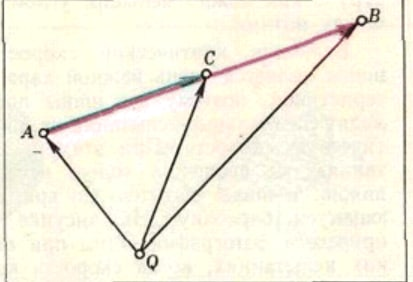
\includegraphics[scale=1.25]{asd.jpg}
\end{multicols}
 \end{small}

\end{document}
